\begin{tikzpicture}[scale = 1.5]
    \draw[rounded corners = 5pt, cyan!50!blue] (0,0) node[above]{$\tilde{\calU}(L,\omega)$};
    

    \draw[->, rounded corners = 5pt] (0,0) --++ (1,0) --++ (0,1) --++ (0.5,0); % (1.5,1)
    \draw[color = blue,fill = white, rounded corners = 2pt] (1.5,0.625) rectangle (3,1.375) node[midway]{$\delta_1$CDC};

    \draw[->] (3,1) --++ (0.5,0);
    \draw[->, rounded corners = 5pt] (3.375,1) --++ (1.25,0); % (4.625,1)
	\draw[->, rounded corners = 5pt] (6.5,1) --++ (0.5,0) --++ (0,-1.25);
    \draw[color = gray,fill=white] (3.875,1) circle(0.375);
    \draw[color = gray] (3.875,1) node{PNR};
    \draw[color = red,fill = white, rounded corners = 2] (4.625,0.625) rectangle (6.75,1.375) node[midway]{$(1-\delta_1)$CDC};

    \draw[->, rounded corners = 5pt] (0,0) --++ (1,0) --++ (0.5,0); % (1.5,0)
    \draw[color = blue,fill = white, rounded corners = 2] (1.5,-0.375) rectangle (3,0.375) node[midway]{$\delta_2$CDC};
    
    \draw[->] (3,0) --++ (0.5,0);
    \draw[->, rounded corners = 5pt] (3.375,0) --++ (1.25,0); % (4.625,0)
    \draw[->, rounded corners = 5pt] (6.5,0) --++ (0.5,0) --++ (0,-1);
    \draw[color = gray,fill=white] (3.875,0) circle(0.375);
    \draw[color = gray] (3.875,0) node{PNR};
    \draw[color = red,fill = white, rounded corners = 2] (4.625,-0.375) rectangle (6.75,0.375) node[midway]{$(1-\delta_2)$CDC};
	

    \draw[color = white, rounded corners = 2] (1.5,-1.25) rectangle (6.5,-0.75) node[midway, color = black]{$\substack{\bullet\\ \bullet\\ \bullet}$};
	
    \draw[->, rounded corners = 5pt] (0,0) --++ (1,0) --++ (0,-2) --++ (0.5,0); % (1.5,1)
    \draw[color = blue,fill = white, rounded corners = 2] (1.5,-2.375) rectangle (3,-1.625) node[midway]{$\delta_N$CDC};
    \draw[->] (3,-2) --++ (0.5,0);
    \draw[->, rounded corners = 5pt] (3.375,-2) --++ (1.25,0); % (4.625,1)
    \draw[->, rounded corners = 5pt] (6.5,-2) --++ (0.5,0) --++ (0,0.5);
    \draw[color = gray,fill=white] (3.875,-2) circle(0.375);
    \draw[color = gray] (3.875,-2) node{PNR};
    \draw[color = red,fill = white, rounded corners = 2] (4.625,-2.375) rectangle (6.75,-1.625) node[midway]{$(1-\delta_N)$CDC};

    \draw[->, rounded corners = 5pt] (7,-1.25) --++ (0.625,0); % towards multiply
    \draw[color = gray,fill=white] (7,-1.25) circle(0.25);
    \draw (7,-1.25) node{$\bm{+}$};
	
\end{tikzpicture}
